\subsection{Architektur}
\label{subsec:architecture}

Die Entwicklung eines Softwaresystem ist ein komplexes Unterfangen und oft nicht mehr überschaubar.
Daher wollen wir bei der Darstellung der Architektur auf einer Makroebene beginnen und nachfolgend einige Details beleuchten.
Am Ende soll dadurch ein detailliertes Verständnis der Anwendung möglich sein.

\subsubsection{Makrosicht}
\label{subsubsec:macro-view}

Unter der Makrosicht der Architektur, wie in Abbildung~\ref{fig:macro-view-diagram} dargestellt, verstehen wir eine grobe Ansicht der verwendeten Komponenten des Softwaresystems.

\begin{figure}[h]
    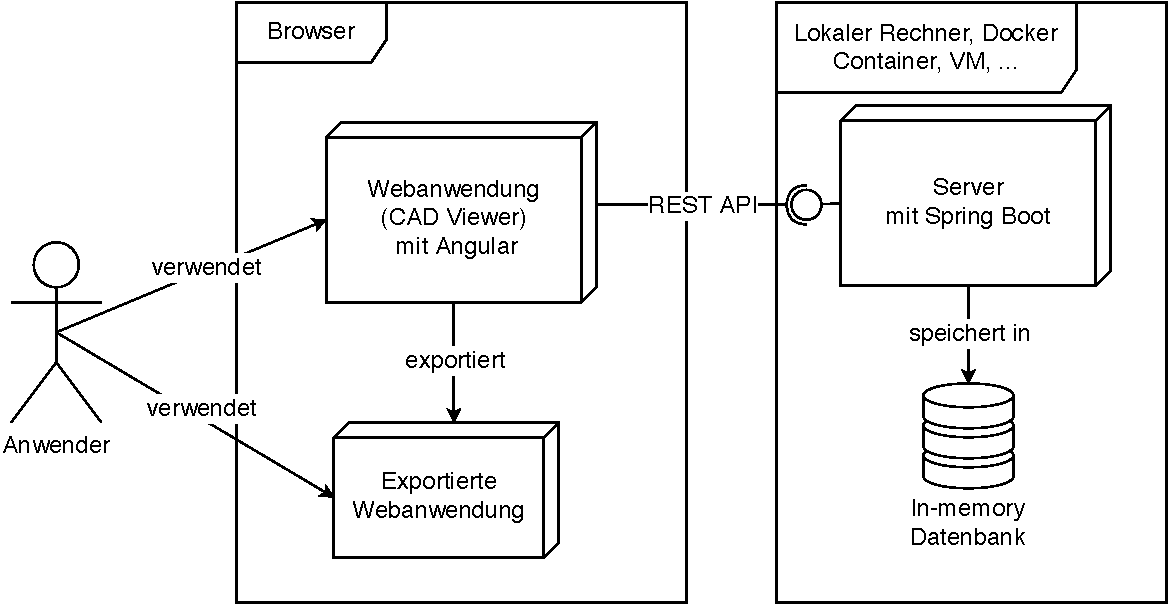
\includegraphics[width=0.5\textwidth]{res/macro.pdf}
    \caption{Darstellung der Makrosicht der Anwendungsarchitektur.}
    \label{fig:macro-view-diagram}
\end{figure}

Die Kernanwendung, der CAD-Viewer, läuft als Webanwendung auf dem Browser des Anwenders.
Wir haben uns dazu entschieden, dass die Exportfunktion wiederum dieselbe Webanwendung, nur ohne Serveranbindung und mit eingebetteter CAD-Datei, exportiert.
Daher befindet sich die exportierte Webanwendung ebenso im Bereich des Browsers.

Auf der anderen Seite des Diagramms ist die Serveranwendung zu finden, welche über eine REST-API angesprochen wird.
Der Server stellt neben seinen Schnittstellen auch die Webanwendung bereit.
Ebenso ist eine In-memory Datenbank darunter dargestellt auf welcher die hochgeladenen CAD-Dateien und Raumzuordnungen flüchtig gespeichert werden.
Wir haben uns für eine flüchtige Speicherung entschieden, da aus unserer Sicht kein Mehrwert durch die Persistierung entstünde.
Nichtsdestotrotz kann die verwendete Datenbank auch im Nachhinein mittels Kommandozeilenparameter wie \texttt{--spring.datasource.url} konfiguriert werden~\cite{JDBCSpringBoot}.

Während die Webanwendung klar im Browser des Anwenders läuft, ist das Laufzeitsystem des Servers unbestimmt.
Es kann sich dabei beispielsweise um den lokalen Rechner eines Anwenders handeln, eine VM oder eine Docker Container.

\subsubsection{Detailsicht des Servers}
\label{subsubsec:detail-server}

TODO:
- Persistenz mit JPA beschreiben
- REST-API beschreiben (Export wird später beschrieben im Teil der Webanwendung)

\subsubsection{Detailsicht der Webanwendung}
\label{subsubsec:detail-webapp}

TODO:
- Aufbau der Anwendung (Komponenten) beschreiben
- Exportfunktion beschreiben
